%%%%%%%%%%%%%%%%%%%%%%%%%%%%%%%%%%%%%%%%%%%%%%%%%%%%%%%%%%%%%%%%%%%%%%%%%%%%%%%%
% setup.tex
% Main tex file for setup and content collocation
% For the use of University of Amsterdam
% Information Systems and Data Science students
% Adapted by Riccardo Fiorista (riccardo.fiorista@proton.me)
%%%%%%%%%%%%%%%%%%%%%%%%%%%%%%%%%%%%%%%%%%%%%%%%%%%%%%%%%%%%%%%%%%%%%%%%%%%%%%%%

% Options:
% Choose one of:
%% `is` - Information Systems
%% `ds` - Data Science 
% Add (separated by `,`):
%% `nolinenumbering` - If you want to remove line numbering on submission
%% `draftmargins` - If you would like to give your reviewer more space for comments
%% `nofrontpicture` - If you do not wish to have a graphic on your front-page
%% `nofirstcompanypicture` - If you do not wish to have a graphic on your front-page
%% `nosecondcompanypicture` - If you do not wish to have a graphic on your front-page
\documentclass[ds]{mscthesis}

%%%%%%%%%%%%%%%%%%%%%%%%%%%%%%%%%%%%%%%%%%%%%%%%%%%%%%%%%%%%%%%%%%%%%%%%%%%%%%%%
% DOCUMENT METADATA
%%%%%%%%%%%%%%%%%%%%%%%%%%%%%%%%%%%%%%%%%%%%%%%%%%%%%%%%%%%%%%%%%%%%%%%%%%%%%%%%

% Thesis related entries
\title{Fill In Your Title}
\subtitle{Fill In Your Sub-Title}

% Date on which your thesis is submitted
\date{Fill In The Date In Format DD.MM.YYYY}

% 4-5 keywords should do the trick. They should ideally be phrases of 2-4 words or single words.
\keywords{keywords, belong, here, with, commas, like, this}

% Author data
\authorname{Your Name}
\authorid{Your Student ID}
\authoremail{your@student.mail}

% Supervisors
\uvasupervisorname{UvA Supervisor}
\uvasupervisoraffiliation{UvA Supervisor}
\uvasupervisoremail{supervisor@uva.nl}

% Comment if you do not have an external supervisor
\externalsupervisorname{External Supervisor} \externalsupervisoraffiliation{External Supervisor}
\externalsupervisoremail{supervisor@company.nl}

% % Uncomment and fill paths if you want to add custom images
% %% Figure size suggestions (in general it's best to render them from SVGs):
% %% 3000x3000 @ 240dpi for all three
% \titlepicturepath{}
% \firstcompanypicturepath{}
% \secondcompanypicture{path}

%%%%%%%%%%%%%%%%%%%%%%%%%%%%%%%%%%%%%%%%%%%%%%%%%%%%%%%%%%%%%%%%%%%%%%%%%%%%%%%%
% CONTENT
%%%%%%%%%%%%%%%%%%%%%%%%%%%%%%%%%%%%%%%%%%%%%%%%%%%%%%%%%%%%%%%%%%%%%%%%%%%%%%%%

\begin{document}
\pagestyle{plain}

\maketitlepage
\fixemptypage
\setcounter{page}{0}

\begin{abstract}
% A summary of results should be included. Avoid citations. Maximum length is 200 words.
Write your abstract here.
\end{abstract}

\maketitle

\section*{Github Repository}
\url{https://github.com/you/your_awesome_thesis_repo}

% Sections; Try to stick to this setup but you can comment each section
\section{Introduction}
\label{sec:introduction}
% Mention scientific context/field, problem statement, research gap and candidate (sub) research question(s). 
Write your introduction here. It should be immediately clear how your proposed contribution is scientifically relevant and fills the research gap.
 \TODO{This is a TODO} This is a test citation \cite{Gruber1995}

Towards the end of the introduction, you should also add your \textit{preliminary} \textbf{reasearch questions (RQ)} here. You may want to state your main RQ like this:

\noindent\textit{To what extent can a master thesis template enhance the quality of the final thesis?}\REMARK{This is a remark}

You can then list the sub-questions as:
\begin{itemize}
    \item How does the structure of the template influence the final grading?
    \item To what extent is textual guidance sufficient for structured working?
    \item \dots
\end{itemize}
\section{Related Work}
\label{sec:related_work}
This thesis aims to address the existing research gap concerning the potential for automatically refactoring EPUBs to enhance their accessibility. This section will explore the current research surrounding this topic by focusing on three topics. The first subsection will explore the most recent issue of the WCAG due to its strong ties to the EPUB Accessibility standard. The subsequent subsection will then discuss the additions that the EPUB Accessibility standard brings on top of the WCAG. The last subsection will focus on current methods for automatically increasing web content accessibility.

Since this is a new field of research, related work on this topic is sparse. Few research articles exist with a similar goal of increasing accessibility automatically. The foundational concepts and theories on the subject of EPUB accessibility will be discussed and related to the subject of web content accessibility. If we know how EPUB accessibility relates to web content accessibility, we can apply the techniques used for automating web content accessibility on EPUBs. These techniques will underpin the chosen methods in this thesis and later, will help answer the three methodological subquestions.


\subsection{Web Content Accessibility Guidelines}
Before we can go in-depth on the specifications of the EPUB Accessibility standards, the WCAG is discussed first. The most recent version of the Web Content Accessibility Guidelines at the time of writing is 2.2. It is important to note that each version since 2.0 does not replace the old version, but rather adds additional guidelines on top of the former version. For version 2.2, this means that nine new success criteria were added compared to 2.1 \cite{WCAGGuidelines}. The WCAG consists of four main principles: Perceivable, Operable, Understandable, and Robust \cite{Caldwell2008}. Since new versions only apply incremental changes, the base structure and principles behind WCAG 2 have remained the same \cite{WCAGGuidelines}.

\textit{Perceivable} is the first principle listed by the WCAG and lays its focus on pursuing perceivable UI components and other web content. This includes guidelines, such as providing alternative text for images, making content distinguishable through color or contrast, and captions for time-based media \cite{Caldwell2008}.

Secondly, the WCAG states that navigating the web content and other UI components must be \textit{operable} to all. This principle is comprised of being able to control the web content by keyboard alone, providing enough time for users to read all text, and not having flashing elements that can cause a seizure \cite{Caldwell2008}.

The third principle of the WCAG is \textit{understandable}. This principle states that UI components and information on the page should be understandable for each user. This means, for example, that the web page should operate predictably to the user's input and that input fields are labeled when input is required \cite{Caldwell2008}.

Lastly, it is stated that content must be \textit{robust} to changes in order to be able to be offered to all users. This includes the usage of assistive technologies that rely on the inner structure of the HTML files that make up the EPUB. This means that each element has opening and closing tags (e.g. <p> and </p>), and that all IDs are unique \cite{Caldwell2008}.

The WCAG also specifies conformance levels. These levels are A, AA, and AAA, increasing in level of accessibility demands. While level A is considered to be the minimum required level, it remains deficient in meeting the expectations of users with disabilities significantly. This is why level AA is generally used as the standard of accessibility \cite{KBDaisyWCAG}. The AAA conformance level does not fall within the scope of this thesis. This level includes success criteria such as prerecorded sign language, making this widely regarded to not be essential in providing good accessibility, while still being good practice for accessible publications \cite{WCAGGuidelines, KBDaisyWCAG}.



\subsection{The EPUB Accessibility standard}
Flowing forth from the WCAG, the EPUB Accessibility standard arises. The first 1.0 specification appeared on the 5th of January 2017 under the name of the IDPF; just weeks before this foundation was absorbed into the W3C. The current EPUB Accessibility 1.1 specification, which came out on the 25th of May 2023, was then also released under the W3C name. This ties it strongly to the WCAG, which is developed by the same entity. The standard was developed in strong collaboration with the creators of the Ace checker, the DAISY consortium.

In relation to the WCAG, the EPUB Accessibility standard holds many of the same core values. One of the main requirements in the EPUB Accessibility standard is that EPUBs must conform to at least the WCAG 2.0 A conformance level \cite{EPUBGuidelines}. Since the WCAG already describes web content accessibility, the additions of the EPUB Accessibility standard focus on what further requirements are needed when it comes to collections of web documents \cite{EPUBGuidelines}. The first requirement is that text-audio playback should be synchronized. This specific requirement falls outside of this thesis' scope, as we do not focus on the auditory experience \cite{EPUBGuidelines}. 

The second requirement is proper page navigation. These should be in place so that a visually impaired person can still easily jump from page to page. Proper page navigation consists of page breaks indicating a new page that are structured in a page list. The page list forms the main way of navigating the EPUB for a visually impaired person. Lastly, the pagination source should be defined, which helps the user identify from where the page breaks originate; for example a specific edition of the book \cite{EPUBGuidelines}. These two requirements combined, form the main addition to the WCAG.



% \subsection{Manual methods of EPUB accessibility enhancement}
% - Look at maybe manual methods? What do they do? and can we take from it?

% This subsection could be before or after the next one



\subsection{Automatic methods for web accessibility}
This subsection will explore the existing literature on automatically improving accessibility on web pages. Since EPUBs are in essence a collection of (X)HTML files, this is the closest relevant and related research in this area. This thesis builds on this existing literature, as it is the current state-of-the-art for any automatic methods of improving web content accessibility. Furthermore, these articles will be used to compare our results to at the end of this thesis.

Ferati \& Sulejmani propose possible techniques for automatically improving accessibility on web pages\cite{Ferati2016}. Their research poses an automated tool that focuses on employing three techniques. Firstly, link enrichment is used to detect if a hyperlink is missing an appropriate label and adds an \textit{aria-labelledby} attribute to the link in order to make it visible for screen readers \cite{Ferati2016}. Furthermore, the image enrichment step provides alt-text to images that do not have that already. On images that contained text, Optical Character Recognition was applied to generate alt-text. In case Optical Character Recognition was not applicable to an image, the Google Image API was used to fetch the description of similar images \cite{Ferati2016}. Lastly, Ferati \& Sulejmani applied navigation enrichment, which skips the navigation bar at the top of a web page. This way, screen readers will not continually repeat the navigation bar each time the page is reloaded \cite{Ferati2016}. All techniques use a form of HTML refactoring to apply the accessibility changes to the web page. This combination of techniques was able to resolve 48\% of all target errors \cite{Ferati2016}.

Another approach is proposed by Ikhsan \& Candra, employing an automatic refactoring method \cite{Ikhsan2018}. Their approach consisted of a small number of steps, keeping the overall process simple. First, certain HTML tags were found using the proprietary HTML Code Sniffer. Then, this HTML tag would be checked for a certain condition. If this condition is met, the tag is compliant, otherwise, a pre-defined solution is applied to this tag. An example of such a condition is: if a \texttt{<head>} tag is found without a title attribute, this attribute is created and added to the  \texttt{<head>} tag\cite{Ikhsan2018}. This reduced the number of errors by between 53.6\% and 98.2\% depending on the website \cite{Ikhsan2018}. However, the research does not mention how, for instance, the content of the title attribute is created. It is thus possible that the overall accessibility of the web page did not improve significantly, in defiance of the significant reduction in errors.

Lastly, Zhang et al. make use of the Beautiful Soup 4 (BS4) library in their approach. The objective of their research is to make SVG buttons on web pages more accessible by providing alt-text \cite{Zhang2024}. One of the challenges that Zhang et al. faced, was that the SVG buttons are hard to identify on a web page. This specific challenge was tackled using BS4, employing its ability to find all potential SVG elements, and then sifting through these to find the legitimate SVG button. This strategy made it possible to provide alt-text to SVG buttons. The refactoring approach of Zhang et al. reduced the amount of their target error by 91.9\% \cite{Zhang2024}.
\section{Methodology}
\label{sec:methodology}
% Focus on what you add to the existing method. Explain what you will do and why (and how). Do not forget to characterize your research design. There should be a sub-section on the evaluation. 
%For DS students, this normally means using manually labelled or ground truth data. For IS students, it is not always needed to have a separate methodology section. You can also integrate the approach with the results in one section. It depends on your type of research what is best fitting.
Write about your methodology here. Focus on your own contribution. Indicate exactly how you will assess your work in terms of evaluation.

% It is possible to use a separate section for the Experimental Setup, which then focuses on all settings used in your experiments. It also possible to address the settings in a sub-section under Methodology. 
\section{Results}
\label{sec:results}
% Give the outcomes for each research question in the form of a table or graphic (with caption).
Write about your results here. Good captions to tables and/or figures are key.

% Sometimes,  especially  if  you  have  quite  different experiments or research  questions,  it makes sense to interleave the experimental setup and the results sections, so the reader does not get lost. It is then helpful to structure clearly in (sub)subsections.
\section{Discussion}
\label{sec:discussion}
% Compare your results with the state-of-the-art and reflect upon the results and limitations of the study. You can already hint at future work to which you come back in the conclusion section.
Write your discussion here. Do not forget to use sub-sections. Normally, the discussion starts with comparing your results to other studies as precisely as possible. The limitations should be reflected upon in terms such as reproducibility,  scalability,  generalizability,  reliability  and  validity. It is also important to mention ethical concerns.
\section{Conclusion}
\label{sec:conclusion}
% Answer each research question and address how the limitations of the study qualify the conclusion.
Write your conclusion here. Be sure that the relation between the research gap and your contribution is clear. Be honest about how limitations in the study qualify the answer on the research question.

\bibliographystyle{ACM-Reference-Format}
\bibliography{bibliographies/references}

\newpage
% You can choose whether you prefer a single or double column appendix.
% Whatever you choose, you will need to stick to it throughout the appendix.
% For double column style, comment the next line.
\onecolumn

\appendix
\begin{appendices}

\section{Appendix}
\label{sec:apx:first_appendix}

\begin{figure}[h]
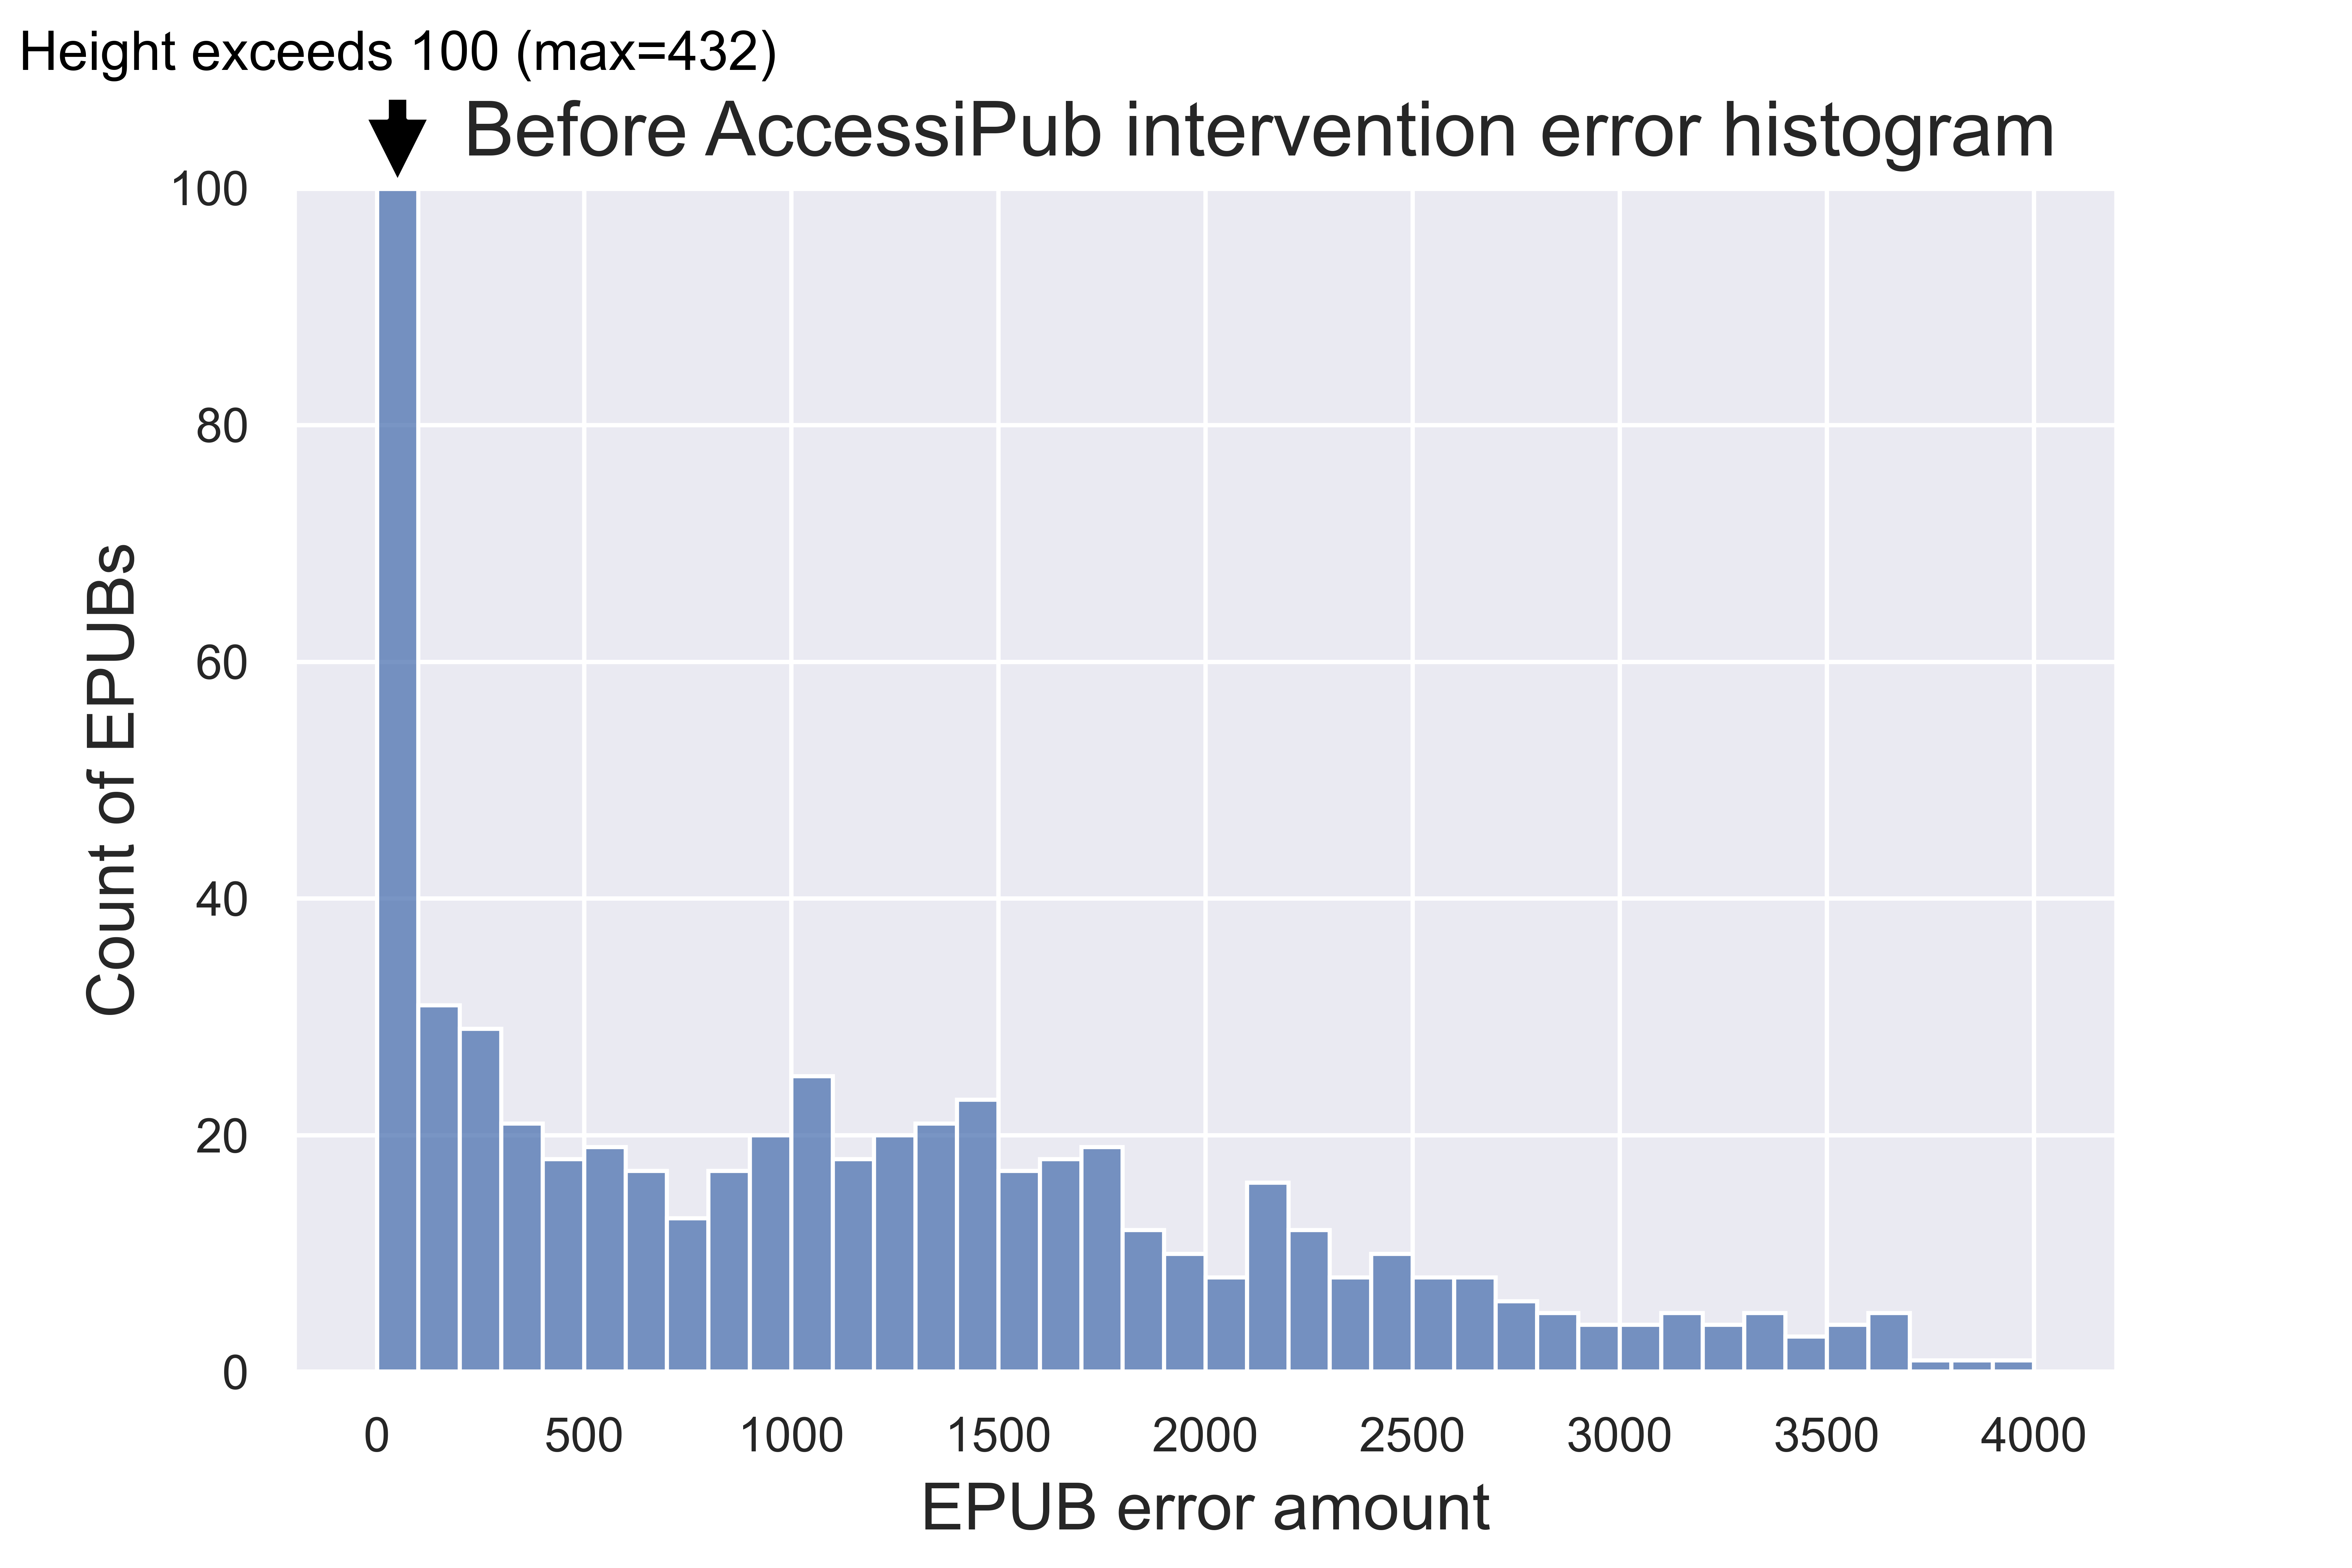
\includegraphics[width=0.48\textwidth,keepaspectratio]{media/images/preaccessipub.png}
\caption{Distribution histogram of the amount of EPUBs per error count before AccessiPub intervention}
\centering
\label{figure:Appendix_pre}
\end{figure}

\begin{figure}[h]
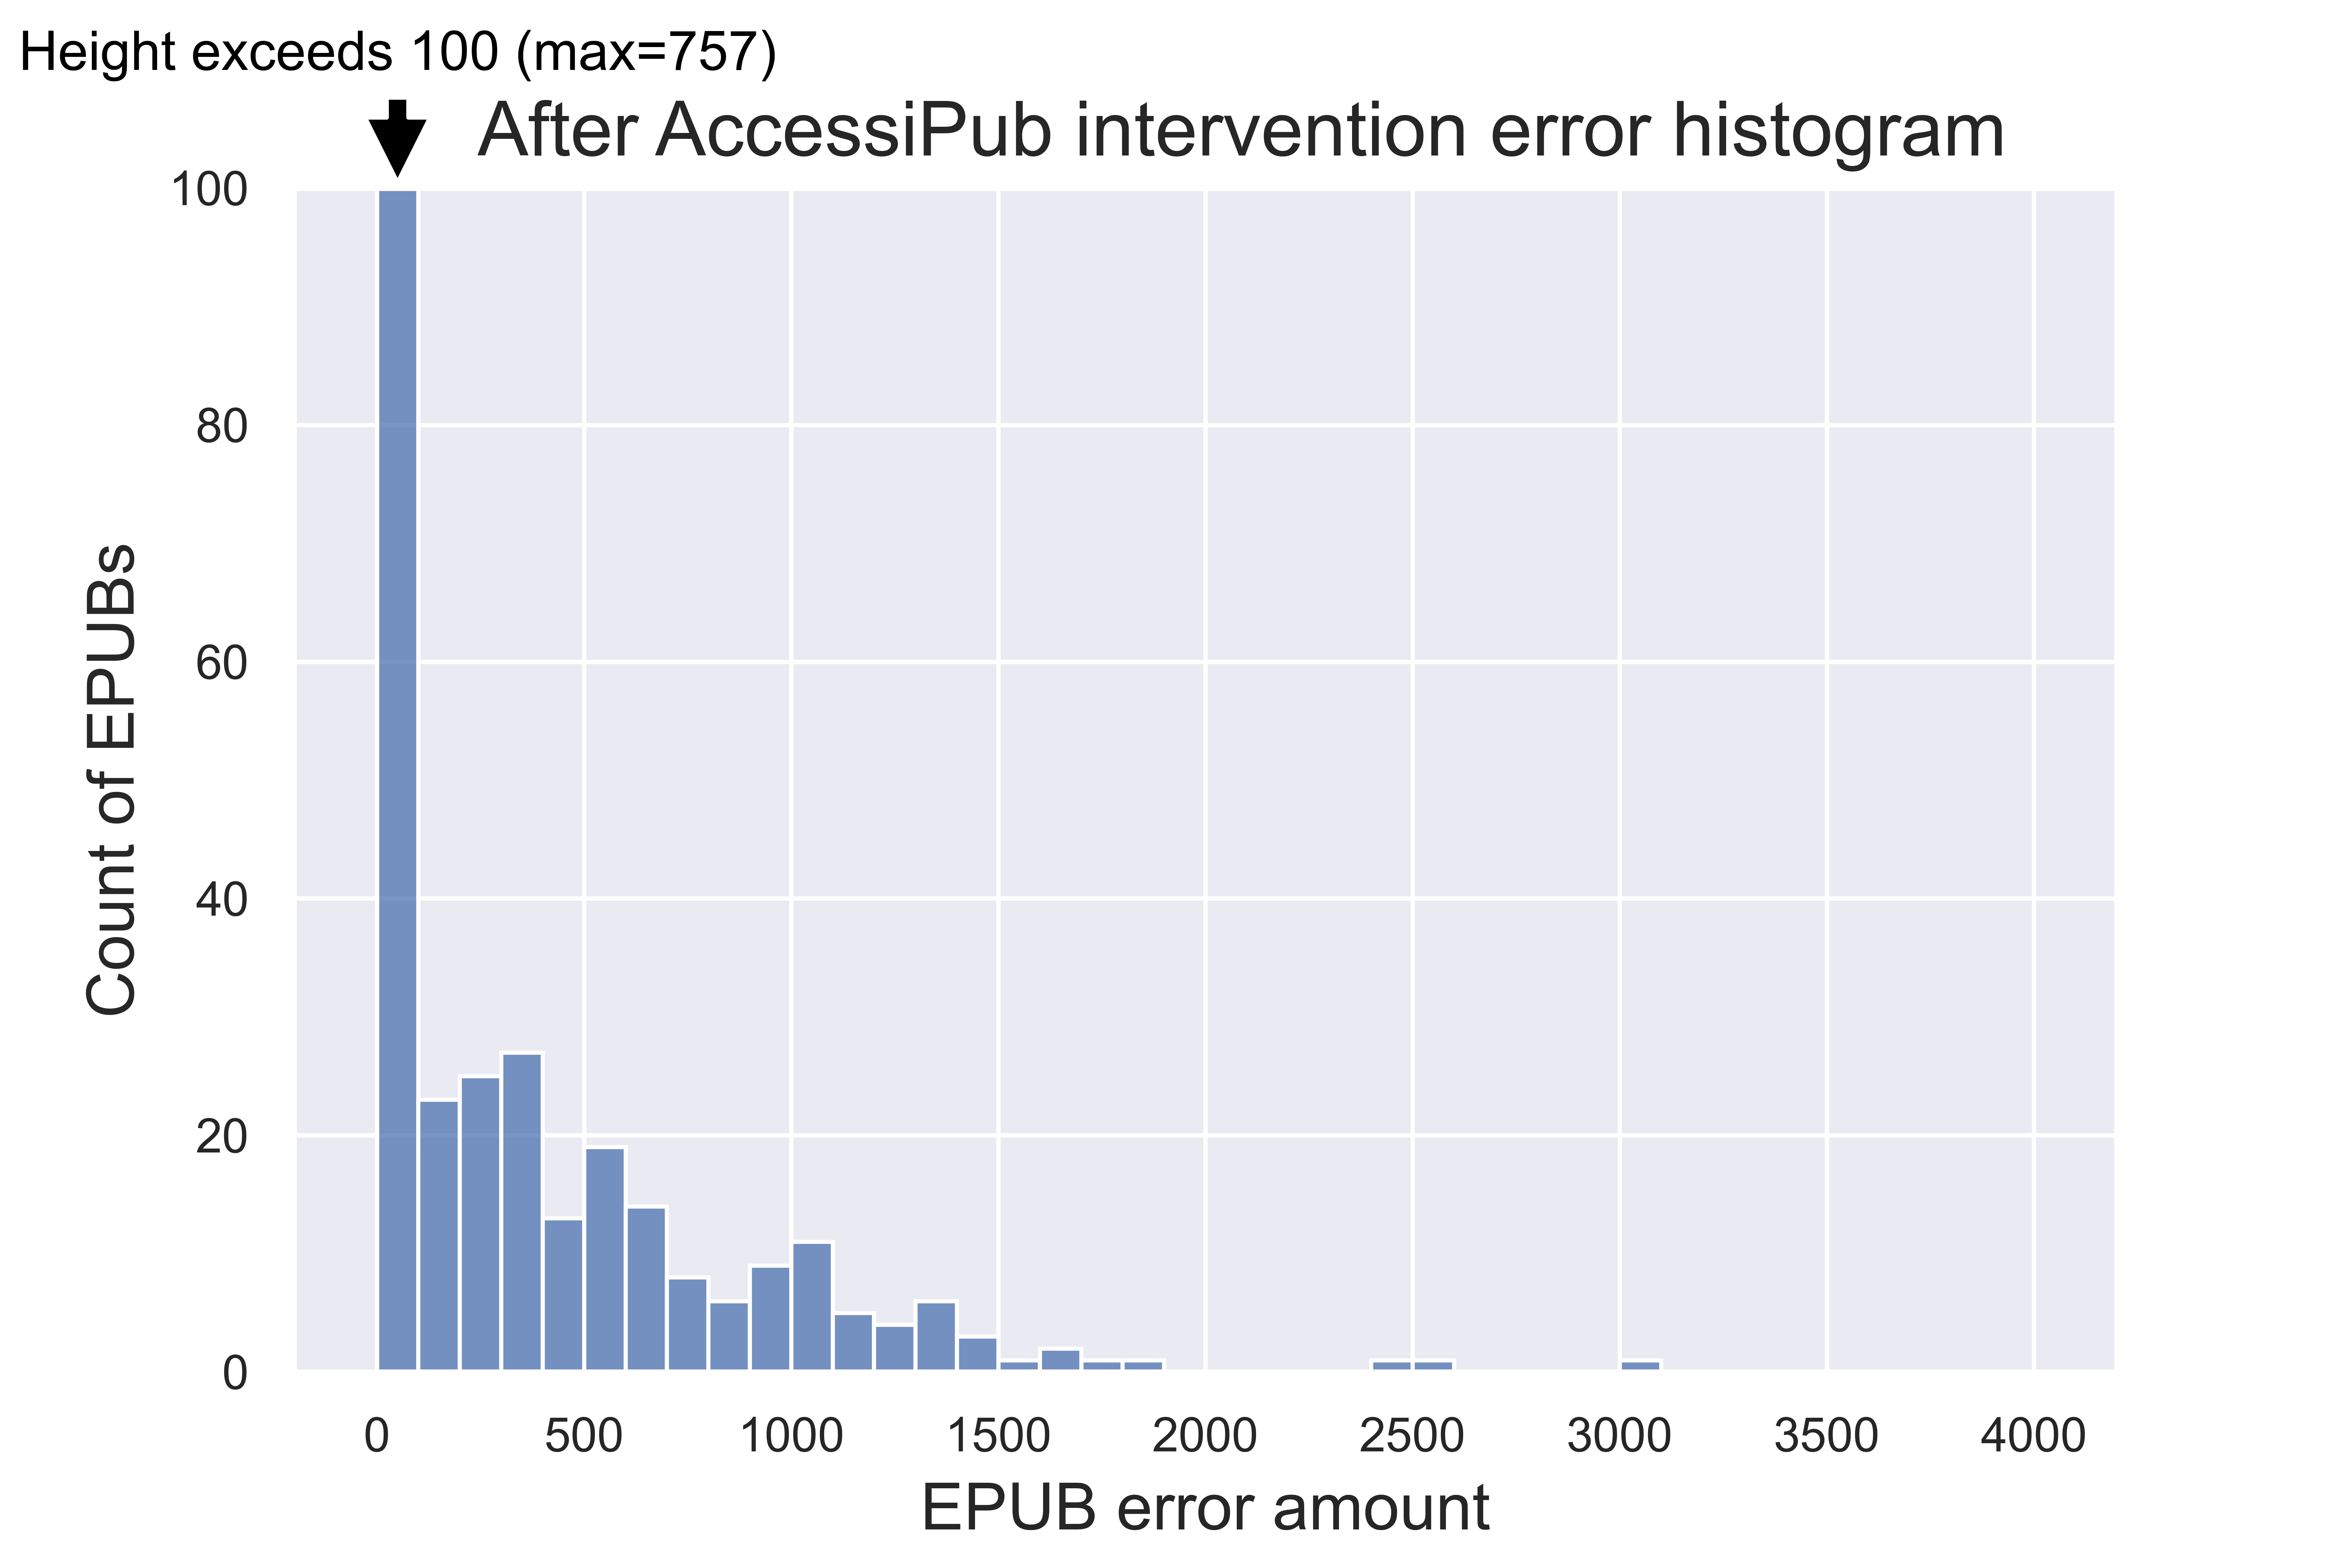
\includegraphics[width=0.48\textwidth,keepaspectratio]{media/images/postaccessipub.png}
\caption{Distribution histogram of the amount of EPUBs per error count after AccessiPub intervention}
\centering
\label{figure:Appendix_post}
\end{figure}

\begin{figure}[h]
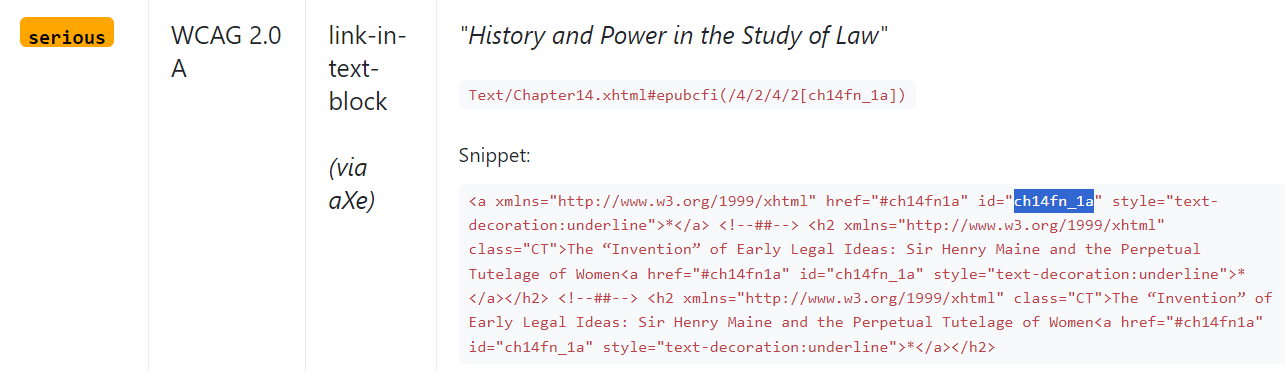
\includegraphics[width=0.72\textwidth,keepaspectratio]{media/images/ace-wrong.png}
\caption{Example 1a: Ace HTML report showing an unjustified link-in-text-block error}
\centering
\label{figure:Appendix_ace-wrong}
\end{figure}

\begin{figure}[h]
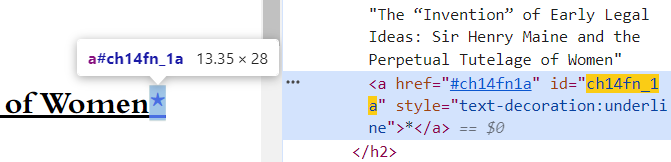
\includegraphics[width=0.72\textwidth,keepaspectratio]{media/images/ace-wrongv2.png}
\caption{Example 1b: Actual rendered HTML file showing an accessible link and showing that the Ace report is false}
\centering
\label{figure:Appendix_ace-wrong_code}
\end{figure}

\begin{figure}[h]
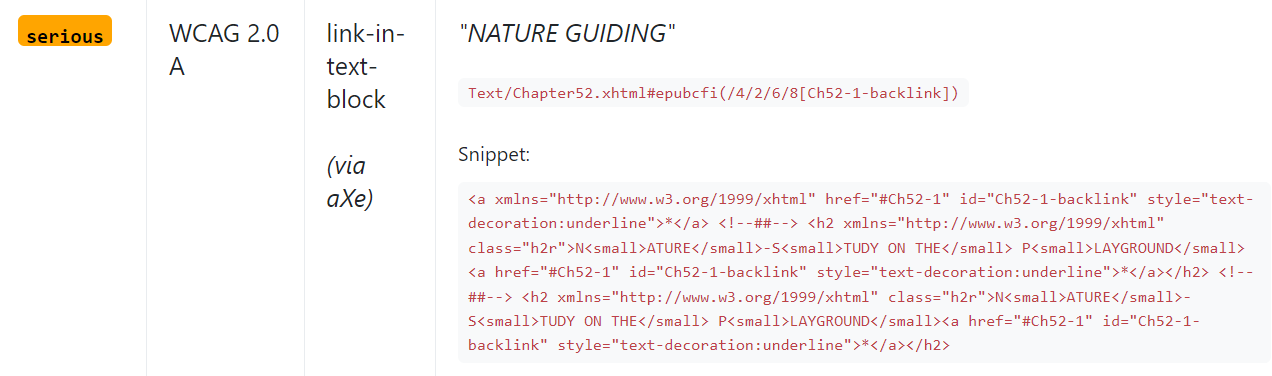
\includegraphics[width=0.72\textwidth,keepaspectratio]{media/images/again-ace-wrong.png}
\caption{Example 2a: Ace HTML report showing an unjustified link-in-text-block error}
\centering
\label{figure:Appendix_ace-wrong2}
\end{figure}

\begin{figure}[h]
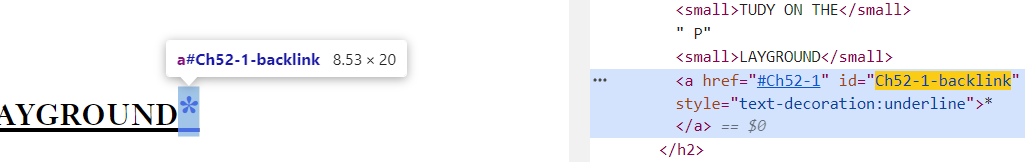
\includegraphics[width=0.72\textwidth,keepaspectratio]{media/images/again-ace-wrongv2.png}
\caption{Example 2b: Actual rendered HTML file showing an accessible link and showing that the Ace report is false}
\centering
\label{figure:Appendix_ace-wrong2_code}
\end{figure}

\end{appendices}

\end{document}

%%%%%%%%%%%%%%%%%%%%%%%%%%%%%%%%%%%%%%%%%%%%%%%%%%%%%%%%%%%%%%%%%%%%%%%%%%%%%%%%
%%%%%%%%%%%%%%%%%%%%%%%%%%%%%%%%%%%%%%%%%%%%%%%%%%%%%%%%%%%%%%%%%%%%%%%%%%%%%%%%